\begin{frame}
    \frametitle{\problemtitle}

    \begin{columns}
        \begin{column}[T]{\textwidth}
            \begin{itemize}
                \item Solve a sliding puzzle with size $h,w \le 500$, where some tiles are glued.
                \item The empty square is at the bottom right position.
                \item Every glued tile is in its correct position.
                \item For each tile that can move, it is possible to have
                the empty square in its position instead.
                \item No glued tiles are encircled by tiles that can move.
                \item All tiles have distinct numbers on them, which must be sorted in ascending order.
            \end{itemize}

            \vspace{1em}

            \small
            \begin{minipage}[t]{.3\textwidth}
                \centering
                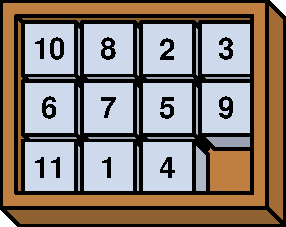
\includegraphics[width=0.6\textwidth]{puzzle.pdf} \\
                Example of a 3-by-4 sliding puzzle, corresponding to Sample~Input~1.
            \end{minipage}
            \hfill
            \begin{minipage}[t]{.3\textwidth}
                \centering
                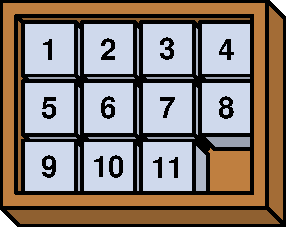
\includegraphics[width=0.6\textwidth]{solvedpuzzle.pdf} \\
                The same sliding puzzle, after solving.
            \end{minipage}
            \hfill
            \begin{minipage}[t]{.3\textwidth}
                \centering
                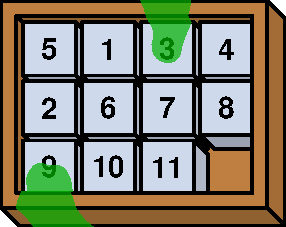
\includegraphics[width=0.6\textwidth]{gluedpossible.pdf} \\
                Example of a sliding puzzle with glued tiles,
                    covered in green goo.
                    This example is possible to solve, corresponding to Sample Input 3.
            \end{minipage}
        \end{column}

        %\illustration{0.25}{illustration.jpg}{
        %    Caption of the illustration (optional).
        %    CC BY-SA 4.0 by X on \href{https://example.com/reference-to-image}{Y}
        %}
    \end{columns}
\end{frame}
